
\chapter{提案手法}
\label{chap:proposed}

%----------------------------------------------
\section{まえがき}
%----------------------------------------------
前章では,FDICAに伴い生じるパーミュテーション問題と従来の深層パーミュテーション解決法について説明した.
本章では,組み合せ爆発を起こすことのない,DNNを用いたデータ駆動型パーミュテーション解決法を新たに提案する.
\ref{sec:moti}節では,IVAやILRMAのようなブラインド(教師無し)なパーミュテーション解決法における課題と従来の深層パーミュテーション解決法における課題を述べ,データ駆動型の教師ありパーミュテーション解決法を新たに提案する動機について明らかにする.
\ref{sec:in-out}節及び\ref{sec:model}節で,提案パーミュテーション解決法におけるDNNモデルの入出力及び構造を説明する.
\ref{sec:loss}節及び\ref{sec:maj}節では,誤差逆伝播に用いる損失の取り方とパーミュテーション行列の並び替えに用いるラベルの取得方法を説明する.
\ref{sec:3matome}節で本章のまとめを述べる.

%----------------------------------------------
\section{動機}
\label{sec:moti}
%----------------------------------------------
%%%%%%%%%%%%%%%%%%%%%%%%%%%%
\begin{figure}[t]
    \begin{center}
        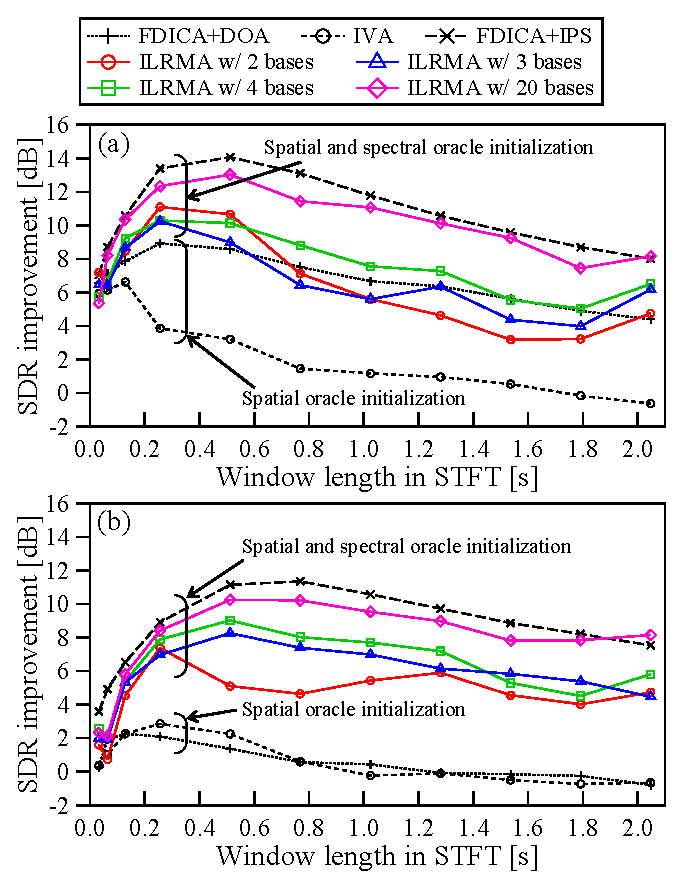
\includegraphics[width=0.8\columnwidth]{figures/SpeechE2AJR2_opt12+note.eps}
    \end{center}
    \vspace{-8pt}
	\caption{Average source separation results for speech signals using random initialization: (a) E2A ($T_{60}$ =$300$~ms) and (b) JR2 ($T_{60}$=$470$~ms) impulse responses~\cite{EU}.}
	\label{fig:kitamura_es}
\end{figure}
%%%%%%%%%%%%%%%%%%%%%%%%%%%%

文献~\cite{EU}では,BSSのSTFTにおける最適な窓長を実験的に検討している.
Fig.~\ref{fig:kitamura_es}(b)は,文献~\cite{EU}の実験結果の図を引用したものである.縦軸は信号対歪み比(source-to-distortion ratio: SDR)\cite{BSSEval}の改善量であり,これは即ち分離性能を表している.この結果より,IVA及びILRMAでは,残響状態$T_{60} = 470~\mathrm{ms}$の条件では分離に失敗していることが分かる.
一方で,FDICAに対して,音源信号$\bm{s}_{ij}$を用いる理想的なパーミュテーション解決法(ideal permutation solver: IPS)を適用した結果では10~dB以上のSDRの改善を達成している.
この事実は,高残響下での音声混合信号であっても,$\hat{\bm{W}}_i$はFDICAで正確に推定でき,$\bm{P}_i^{-1}$の推定のみ失敗していることを示している.
また,従来の深層パーミュテーション解決法では,全周波数帯域中の局所的な狭帯域のおけるパーミュテーション問題の解決を全時間方向と全周波数方向に行う際に,ある参照周波数に対して同一か否かで音源を判断しているため,3音源以上の分離等の拡張性に欠ける.
そこで,本論文では,簡潔なアルゴリズムでパーミュテーション問題を正確に解くことに焦点を当て,新しいDNNに基づくデータ駆動型(教師あり)パーミュテーション解決法を提案する.
以後,本論文では,提案するパーミュテーション問題の解決法が実現可能かどうかを判断するために,FDICAを適応した後の分離信号に模倣した人工データと実際の音声データを用いてパーミュテーション問題の解決を考える.この際,音源数$N=2$及びチャネル数$M=2$と仮定し,実験を行う.
提案するパーミュテーション解決法の概要は以下の通りである.
\begin{itemize}
    \item 分離信号$\bm{Y}_1$及び$\bm{Y}_2$から全周波数成分の値を保持するミニ振幅スペクトログラムを取り出し,それぞれに対して全ての音源のパワースペクトログラムの値を基準にして正規化を行った値をDNNに入力する
    \item DNNは入力された2つのミニ振幅スペクトログラムの値がどの音源の値かを予測し,$0$〜$1$の間の確率値として出力する
    \item DNNから出力された確率値に従ってシャッフルされたスペクトログラムを並び替えた行列と,完全に分離されたスペクトログラムとの間で損失を取得する
    \item $\bm{Y}_1$及び$\bm{Y}_2$の全時間方向に対してDNNが適用される
    \item 最終的な推定値(ラベル)$\widehat{\bm{L}}$は,予測値の時間方向への多数決結果から決定される
\end{itemize}

提案するパーミュテーション解決法では,全周波数成分を持ったミニ振幅スペクトログラムに対して,どの音源の成分が入っているかをDNNで予測し,その予測結果に基づいてパーミュテーション解決を行う.
また,DNNには大量の学習用データが必要であるが,IPSで理想的にパーミュテーション解決された分離信号$\bm{Z}_n$を周波数毎にランダムにシャッフルすることで,容易かつ大量に生成することができる.
%----------------------------------------------
\section{DNNの入出力}
\label{sec:in-out}
%----------------------------------------------

観測された混合信号$\bm{X}_n$にFDICAを適用すると,パーミュテーション問題が生じた分離信号$\bm{Y}_n$が得られる.
DNNへの入力は,各分離信号のパワースペクトログラム成分を全ての分離信号のパワースペクトログラム成分で割った値を用いる.
即ち,2音源の場合DNNの入力に用いる信号成分は次のようになる.

\begin{align}
    \widehat{\bm{Y}}_1  = \frac{|\bm{Y}_1|^2}{|\bm{Y}_1|^2+|\bm{Y}_2|^2}\\
    \widehat{\bm{Y}}_2  = \frac{|\bm{Y}_2|^2}{|\bm{Y}_1|^2+|\bm{Y}_2|^2}
\end{align}
ここで,DNNの入力に用いる値をそれぞれ$\widehat{\bm{Y}}_1~\in \mathbb{R}_{\geq 0}^{I \times J}$,$\widehat{\bm{Y}}_2 ~\in \mathbb{R}_{\geq 0}^{I \times J}$とする.
この時,$i = 1,\ldots,I$及び$j = \tau,\ldots,J-\tau$はそれぞれ全周波数帯域の周波数ビン及び時間フレームのインデクスである.DNNの入力にはミニ振幅スペクトログラムを用いるので,元のスペクトログラムの値からはみ出ることがないように$j$の範囲を限定的にしている.
ここで,行列の $|\cdot|^{.2}$ は,要素ごとの絶対値の二乗を示す.時間フレーム$j$における分離信号を次式で表す.

\begin{align}
    \widehat{\bm{y}}_{1j}  = [\widehat{y}_{11j},y_{12j}, \cdots, \widehat{y}_{1Ij} ]^\mathrm{T}\\
    \widehat{\bm{y}}_{2j}  = [\widehat{y}_{21j},y_{22j}, \cdots, \widehat{y}_{2Ij} ]^\mathrm{T}
\end{align}

ここで,$\widehat{y}_{1ij}$は$\widehat{\bm{Y}}_1$の$ij$要素であり,$\widehat{y}_{2ij}$は$\widehat{\bm{Y}}_2$の$ij$要素を表す.
DNNの入力として与える情報は,$j$近傍の時間フレームの列ベクトルを結合したベクトルとする.
これを$\bm{x}_j$とおくと,次式のように構成される.また,$j$近傍の時間フレームの幅は$\tau$とする.
\begin{align}
    \bm{x}_j = [\widehat{\bm{y}}_{1 (j-\tau)}^\mathrm{T}, \cdots,\widehat{\bm{y}}_{1 (j+\tau)}^\mathrm{T}, \widehat{\bm{y}}_{2 (j-\tau)}^\mathrm{T},\cdots,\widehat{\bm{y}}_{2 (j+\tau)}^\mathrm{T} ]^\mathrm{T}
\end{align}

Fig.~\ref{fig:DNN_input}に示すように,上記の$\bm{x}_j$がDNNの入力ベクトルとなる.

%%%%%%%%%%%%%%%%%%%%%%%%%%%%
\begin{figure}[t]
    \begin{center}
        \includegraphics[width=0.8\columnwidth]{figures/DNN_input.pdf}
    \end{center}
    \vspace{-8pt}
	\caption{Input vector of DNN.}
	\label{fig:DNN_input}
\end{figure}
%%%%%%%%%%%%%%%%%%%%%%%%%%%%

\begin{align}
    \bm{L} = \mathrm{DNN}(\bm{x}_j)
\end{align}

DNNが出力する予測は$\bm{L} ~\in \mathbb{R}_{[0,1]}^{2 \times I}$であり,確率値を示す.
$\bm{L}$の1行目には,各周波数成分における音源1である確率値,2行目には,各周波数成分における音源2である確率値が代入される.

\begin{align}
    \bm{L} &= [\bm{l}_{1} , \bm{l}_{2}]^\mathrm{T}\\
    \bm{l}_n &= [\widehat{l}_{n 1}, \cdots, \widehat{l}_{n I}]^\mathrm{T}
\end{align}


%----------------------------------------------
\clearpage
\section{DNNの構造}
\label{sec:model}
%----------------------------------------------
%%%%%%%%%%%%%%%%%%%%%%%%%%%%
\begin{figure}[t]
    \begin{center}
        \includegraphics[width=0.8\columnwidth]{figures/overview_DNN.pdf}
    \end{center}
    \vspace{-8pt}
	\caption{DNN architecture.}
	\label{fig:Dnnmodel}
\end{figure}
%%%%%%%%%%%%%%%%%%%%%%%%%%%%

Fig.~\ref{fig:Dnnmodel}に提案手法のDNNの構造を示す.
提案するDNNの構造は,入力層,隠れ層3層,及び出力層の計5層からなる全結合構成となっており,1~5番目の隠れ層にはrectified linear unit (ReLU)~\cite{relu} 関数,最終隠れ層にはsoftmax関数を適用している.
各隠れ層の次元数は全て,4096である.

%----------------------------------------------
\section{損失の取り方}
\label{sec:loss}
%----------------------------------------------
誤差逆伝播を行う際の損失は,DNNが出力した確率値に従ってパーミュテーション行列を並び替えた行列と完全に分離された行列との間で平均二乗誤差(mean squared error: MSE)を使用して得る.
\ref{sec:in-out}節より,$\widehat{\bm{l}}_{n}$は,全周波数帯域における音源$n$の成分が含まれる割合で構成されている.
また,次式でパーミュテーション行列の並び替えを行い,予測行列$\widetilde{\bm{Y}}_{1 j} ~\in \mathbb{R}_{\geq 0}^{I \times (2\tau+1)}$と$\widetilde{\bm{Y}}_{2 j} ~\in \mathbb{R}_{\geq 0}^{I \times (2\tau+1)}$の2種類を導く.

\begin{align}
    \widetilde{\bm{y}}_{1 j} &= [{y}_{1 1 j} \widehat{l}_{1 1} + y_{2 1 j} \widehat{l}_{2 1}, \cdots, {y}_{1 I j} \widehat{l}_{1 I} + y_{2 I j} \widehat{l}_{2 I}]^\mathrm{T}\\
    \widetilde{\bm{y}}_{2 j} &= [{y}_{1 1 j} \widehat{l}_{2 1} + y_{2 1 j} \widehat{l}_{1 1}, \cdots, {y}_{1 I j} \widehat{l}_{2 I} + y_{2 I j} \widehat{l}_{1 I}]^\mathrm{T}\\
    \widetilde{\bm{Y}}_{1 j} &= [\widetilde{\bm{y}}_{1 (j-\tau)}, \cdots, \widetilde{\bm{y}}_{1 (j+\tau)}] \\
    \widetilde{\bm{Y}}_{2 j} &= [\widetilde{\bm{y}}_{2 (j-\tau)}, \cdots, \widetilde{\bm{y}}_{2 (j+\tau)}] 
\end{align}
ここで,${y}_{1 i j}$は$\bm{Y}_1$の$ij$要素であり,${y}_{2 i j}$は$\bm{Y}_2$の$ij$要素を表す.
$\widetilde{\bm{Y}}_{1 j} ~\in \mathbb{R}_{\geq 0}^{I \times (2\tau+1)}$,$\widetilde{\bm{Y}}_{2 j} ~\in \mathbb{R}_{\geq 0}^{I \times (2\tau+1)}$と
完全に分離された信号のミニスペクトログラム成分$\bm{Z}_{1 j}~\in \mathbb{R}_{\geq 0}^{I \times (2\tau+1)}$,$\bm{Z}_{2 j}~\in \mathbb{R}_{\geq 0}^{I \times (2\tau+1)}$でMSEを使用し,損失を得る.
また,本論文ではパーミュテーション問題を解くことを考えており,分離信号の順番には触れないため,次式で損失を計算する.

\begin{align}
    \mathrm{Loss} = \mathrm{MIN}\{\mathrm{MSE}(\widetilde{\bm{Y}}_{1 j}, \widetilde{\bm{Z}}_{1 j}) + \mathrm{MSE}(\widetilde{\bm{Y}}_{2 j}, \widetilde{\bm{Z}}_{2 j}) ~ , ~ \mathrm{MSE}(\widetilde{\bm{Y}}_{1 j}, \widetilde{\bm{Z}}_{2 j}) + \mathrm{MSE}(\widetilde{\bm{Y}}_{2 j}, \widetilde{\bm{Z}}_{1 j})\}
\end{align}

DNNは上記のLossを最小化するように学習を行う.これらの処理をFig.~\ref{fig:loss}に示す.最終的なラベル$\widetilde{\bm{L}}$は,$\bm{L}$の列成分を比較し,値が大きい方のインデクスを含んだベクトルとなる.
\begin{align}
    \begin{split}
        \widetilde{l}_i &= \left \{
            \begin{array}{l}
                1~(\widehat{l}_{1i} \leq \widehat{l}_{2i}) \\
                0~(\widehat{l}_{2i} \leq \widehat{l}_{1i})
            \end{array}
        \right.
    \end{split}\\
    \widetilde{\bm{L}} &= [\widetilde{l}_1, \cdots, \widetilde{l}_I]^\mathrm{T}
\end{align}

%%%%%%%%%%%%%%%%%%%%%%%%%%%%
\begin{figure}[t]
    \begin{center}
        \includegraphics[width=1.0\columnwidth]{figures/loss.pdf}
    \end{center}
    \vspace{-8pt}
	\caption{The process of calculating losses.}
	\label{fig:loss}
\end{figure}
%%%%%%%%%%%%%%%%%%%%%%%%%%%%


%----------------------------------------------
\section{時間方向への多数決}
\label{sec:maj}
%----------------------------------------------
%%%%%%%%%%%%%%%%%%%%%%%%%%%%
\begin{figure}[t]
    \begin{center}
        \includegraphics[width=0.9\columnwidth]{figures/majority.pdf}
    \end{center}
    \vspace{-15pt}
	\caption{DNN predictions for all short-time subbands and their majority decision.}
	\label{fig:majority}
	\vspace{-8pt}   % キャプションと本文の間隔微調整用クトル
\end{figure}
%%%%%%%%%%%%%%%%%%%%%%%%%%%%
音声信号は本来,無音区間が多く存在することから,一定区間の長さの成分を持つ$\widehat{\bm{Y}}_1$や$\widehat{\bm{Y}}_2$はほぼ零ベクトルになる可能性があり,その場合DNNの予測は不安定になる.
この問題に対処するために,Fig.~\ref{fig:majority}に示すように,長さ$2\tau+1$の入力ベクトルをストライド幅1でシフトさせて,全時間フレームに対してDNNの予測処理を走査する.
そして,DNNの予測結果を時間軸に関して多数決することで,より信頼性の高いラベル$\widehat{\bm{L}}$ を得る.
この処理は,次のように示される.
\begin{align}
    \widehat{\bm{L}} &= \mathrm{round} \left(\frac{1}{J-13} \sum_{\j} \widetilde{\bm{L}}_{j} \in \{0, 1\}^{I} \right)
\end{align}

$\widehat{\bm{L}}$の値に従って,パーミュテーション行列を並び替えることで,パーミュテーション問題の解決を行う.

%----------------------------------------------
\section{本章のまとめ}
\label{sec:3matome}
%----------------------------------------------
本章では,FDICAのポスト処理としてDNNに基づくパーミュテーション解決法について提案した.
提案手法は,各音源のパワースペクトログラムに対して全ての分離信号のパワースペクトログラムで割ったものをDNNの入力として用いる.また,DNNの出力である確率値を用いてパーミュテーション行列を並び替え,
後に完全に分離されたスペクトログラムとの間でMSEを行うことと,時間方向への多数決処理を用いることで,より精度の高い予測ができる.